%%%%%%%%%%%%%%%%%%%%%%%%%%%%%%%%%%%%%%%%%%%%%%%%%%%%%%%%%%%%%%%%%%%%%%%%%%%%%%
%%% --- Population

%BeginMC
\question
Which of the following is \textit{not} one of the four factors that play a role in population growth rate?

\begin{choices}
\choice Immigration.%EndChoice
\choice Death rate.%EndChoice
\choice Emigration.%EndChoice
\choice Birth rate.%EndChoice
\correctchoice Demography.%EndChoice
\end{choices}
%EndMC



%BeginMC
\question
The difference between emigration and immigration is

\begin{choices}
\correctchoice emigration is when individuals move out of a population; immigration is when individuals move into a population.%EndChoice
\choice the direction in which individuals are moving into or out of the population.%EndChoice
\choice emigration is when individuals move into a population; immigration is when individuals move out of a population.%EndChoice
\choice the overall movement of individuals among populations.%EndChoice
\choice emigration is when individuals move out of a population; immigration is when individuals move out of a community.%EndChoice
\end{choices}
%EndMC

%BeginMC
\question
If immigration is greater than emigration and if the birth rate is greater than the death rate in populations with limited resources, then

\begin{choices}
\correctchoice if nothing changes then the population will eventually reach or exceed the carrying capacity of the environment.%EndChoice
\choice the population has plenty of resources.%EndChoice
\choice the population will experience exponential growth.%EndChoice
\choice the death rate will likely decrease and the birth rate will likely increase.%EndChoice
\choice the number of predators will also increase.%EndChoice
\end{choices}
%EndMC

%BeginMC
\question
If emigration is greater than immigration and if the death rate is greater than the birth rate then

\begin{choices}
\correctchoice the population size will decrease.%EndChoice
\choice the population has plenty of resources.%EndChoice
\choice the population size will increase by exponential growth.%EndChoice
\choice the population size will remain about the same.%EndChoice
\choice the population size will get larger if the birth rate is larger than immigration.%EndChoice
\end{choices}
%EndMC


%BeginMC
\question
Which of the following is the best definition of a population?

\begin{choices}
\choice A group of individuals of the same species living apart in different areas.%EndChoice
\choice Groups of individuals of different species living together in the same area.%EndChoice
\choice Groups of individuals of different species living apart in different areas.%EndChoice
\choice A group of individuals of the same species living together in the same area but not interacting with each other.%EndChoice
\correctchoice A group of individuals of the same species living together in the same area.%EndChoice
\end{choices}
%EndMC


%BeginMC
\question
A 20-year study of gray squirrels observed that the population size decreased during the first 15 years but increased during the last five years. With only this information, which of the following is the best explanation for the observed pattern?

\begin{choices}
\correctchoice The population size at the start of the study was greater than the carrying capacity but the population size eventually fell below carrying capacity. %EndChoice
\choice The population size of squirrel predators increased during the first 15 years and decreased during the last five years. %EndChoice
\choice The effects of a severe drought caused a decrease in the amount of their normal food for 15 years but the squirrels eventually switched to a new food. %EndChoice
\choice The population was part of a trophic cascade. %EndChoice
\choice A better competitor, such as fox squirrels, prevented the gray squirrels from getting all of the food they needed to survive.%EndChoice
\end{choices}
%EndMC

%BeginMC
\question
When the number of organisms in a population remains more or less the same over time in the specific place where these organisms live, then this population has reached the \underline{\hspace{2cm}} of that place.

\begin{choices}
\choice exponential growth capacity%EndChoice
\choice maximum growth capacity%EndChoice
\choice logisitic growth capacity%EndChoice
\correctchoice carrying capacity%EndChoice
\choice population density%EndChoice
\end{choices}
%EndMC

%BeginMC
\question
The type of growth curve shown in the figure below is a

\begin{multicols}{2} 
\begin{choices}
\correctchoice logistic growth curve.%EndChoice
\choice exponential growth curve.%EndChoice
\choice carrying capacity growth curve.%EndChoice
\choice population density growth curve.%EndChoice
\choice maximum growth curve.%EndChoice
\end{choices}
\columnbreak
	\hfill 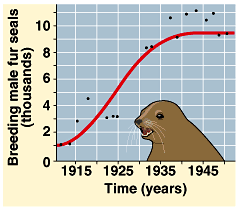
\includegraphics[width=5cm]{img/logistic_growth.png}
\end{multicols}
%EndMC


%BeginMC
\question
A table about a population that lists such items as age, observed number of organisms alive each year, and life expectancy is known as a (an)

\begin{choices}
\choice carrying capacity table.%EndChoice
\choice survivorship table.%EndChoice
\choice exponential growth table.%EndChoice
\choice logistic growth table.%EndChoice
\correctchoice life history table.%EndChoice
\end{choices}
%EndMC

%BeginMC
\question
If a population has passed the carrying capacity of the environment, then which of the following might happen?

\begin{choices}
\choice immigration might increase because fewer individuals will reproduce.%EndChoice
\choice individuals in the population will stop reproducing.%EndChoice
\choice the birth rate will increase to compensate for the increased death rate.%EndChoice
\correctchoice emigration might increase because of limited food supply.%EndChoice
\choice the rate of predation will increase until the population size has fallen below the carrying capacity.%EndChoice
\end{choices}
%EndMC

%BeginMC
\question
Assuming a population has unlimited resources, exponential growth would occur in a population if

\begin{choices}
\correctchoice the immigration rate exceeds the emigration rate and the birth rate exceeds the death rate.%EndChoice
\choice the emigration rate exceeds the immigration rate and the birth rate exceeds the death rate.%EndChoice
\choice the immigration rate exceeds the death rate and the emigration rate is lower than the birth rate.%EndChoice
\choice the immigration rate equals the emigration rate and the birth rate equals the death rate.%EndChoice
\choice the emigration rate exceeds the death rate and the immigration rate is less than the birth rate.%EndChoice
\end{choices}
%EndMC

%BeginMC
\question
Assuming a population has unlimited resources, exponential growth occurs because

\begin{choices}
\correctchoice the birth rate exceeds the death rate.%EndChoice
\choice the emigration rate exceeds the death rate.%EndChoice
\choice the death rate exceeds the birth rate.%EndChoice
\choice the immigration rate equals the death rate and the emigration rate equals the birth rate.%EndChoice
\choice the emigration exceeds the birth rate.%EndChoice
\end{choices}
%EndMC


%BeginMC
\question
You are observing a population of bluebirds when you notice that the number of adults suddenly decreased by 50\% over two days. Which of the following is the most likely explanation for such an observation?

\begin{choices}
\choice decreased birth rate.%EndChoice
\correctchoice increased death rate.%EndChoice
\choice increased immigration.%EndChoice
\choice decreased emigration.%EndChoice
\choice decreased predation.%EndChoice
\end{choices}
%EndMC


%BeginMC
\question
Carrying capacity

\begin{choices}
\choice is seldom reached by most population because the environment has plenty of resources.%EndChoice
\correctchoice is the maximum population size that a particular environment can support.%EndChoice
\choice does not for most species most of the time.%EndChoice
\choice is determined by birth and death rates, and emigration and immigration rates.%EndChoice
\choice describes the stress a population undergoes due to limited resources.%EndChoice
\end{choices}
%EndMC


%%% --- Population END
%%%%%%%%%%%%%%%%%%%%%%%%%%%%%%%%%%%%%%%%%%%%%%%%%%%%%%%%%%%%%%%%%%%%%%%%%%%%%%%%
%%%%%%%%%%%%%%%%%%%%%%%%%%%%%%%%%%%%%%%%%%%%%%%%%%%%%%%%%%%%%%%%%%%%%%%%%%%%%%%%
%%% --- Community

%BeginMC
\question
Forest mice eat seeds. Suppose a fire on the forest floor reduces the amount of seeds by 75\%. The mice survive the fire but what will happen to the size of the mouse population?

\begin{choices}
\correctchoice It will decrease to about 75\% after a delay. %EndChoice
\choice It will decrease rapidly by about 75\%. %EndChoice
\choice It will decrease only a little as mice shift to another food source. %EndChoice
\choice It will increase as the mice shift to another food source. %EndChoice
\choice It will not be affected because mice survived the fire. %EndChoice
\end{choices}
%EndMC



%BeginMC
\question
Bobcats eat forest mice. The mice eat seeds. Suppose a fire on the forest floor reduces the amount of seeds by 75\%.  Before the fire, the population of mice sustained a bobcat population of 8. What will \emph{most likely} happen to the bobcat population as a result of the fire? The bobcat population will

\begin{choices}
\correctchoice decrease to two after a delay. %EndChoice
\choice decrease to two almost immediately. %EndChoice
\choice decrease by two but most will survive. %EndChoice
\choice increase as the bobcats shift to another food source. %EndChoice
\choice not be affected because the mice survived the fire. %EndChoice
\end{choices}
%EndMC


%BeginMC
\question
Species Old can nest anywhere in a certain kind of pine tree. Recently, due to global climate change, Species New has arrived from down south. Species New also nests in the same kind of pine tree. However, Species New can only nest in the outermost parts of any branch (shown in darker color).  Species Old chases away Species New in the inner part of the tree but ignores Species New in the outer part of the tree. What will \emph{most likely} happen in the tree after a few years?

\begin{multicols}{2} 
\begin{choices}
\correctchoice Species New will nest in the outer part of the tree and Species Old will nest in the inner part of the tree.%EndChoice
\choice Species Old will prevent Species New from making nests so Species New will die out in this location.%EndChoice
\choice Species New will prevent Species Old from making nests so Species Old will die out in this location.%EndChoice
\choice Both species will nest in the outer part of the tree in equal numbers but only Species Old will nest in the inner part of the tree.%EndChoice
\choice Species Old will nest more often in the outer part of the tree.%EndChoice
\choice Neither species will survive because they can't nest in the entire tree. %EndChoice
\end{choices}
\columnbreak
	\hfill \includegraphics[width=5cm]{ex3_partition_tree.png}
\end{multicols}
%EndMC




%BeginMC
\question
Which of the following are important biotic (living) factors that can affect the  organization of communities?

\begin{choices}
\choice precipitation, wind%EndChoice
\choice nutrient availability, soil pH%EndChoice
\correctchoice predation, competition%EndChoice
\choice temperature, water%EndChoice
\choice light intensity, seasonality%EndChoice
\end{choices}
%EndMC



%BeginMC
\question
Consider the food chain grass $\to$ grasshopper $\to$ mouse $\to$ snake $\to$ hawk. How much of the chemical energy fixed by photosynthesis of the grass (100\%) is available to the hawk?

\begin{choices}
\correctchoice 0.01\%%EndChoice
\choice 0.1\%%EndChoice
\choice 1\%%EndChoice
\choice 10\%%EndChoice
\choice 60\%%EndChoice
\end{choices}
%EndMC

%BeginMC
\question
Which of the following is \emph{not} directly concerned with community ecology?

\begin{choices}
\choice herbivory%EndChoice
\choice predation%EndChoice
\correctchoice intraspecific competition%EndChoice
\choice resource partitioning%EndChoice
\choice symbiosis%EndChoice
\end{choices}
%EndMC

%BeginMC
\question
The difference between populations and communities is that

\begin{choices}
\correctchoice populations include individuals of the same species; communities include individuals of different species.%EndChoice
\choice populations include individuals of the different species; communities include individuals of the same species.%EndChoice
\hoice populations include interactions between individuals and their physical environment; communities do \emph{not} include such interactions.%EndChoice
\choice populations do \emph{not} include interactions between individuals and the physical environment; communities do include such interactions.%EndChoice
\choice populations are groups of individuals of the same species; communities are groups of communities of the same species.%EndChoice
\end{choices}
%EndMC

%BeginMC
\question
The difference between communities and ecosystems is that

\begin{choices}
\choice communities include individuals of the same species; ecosystems include individuals of different species.%EndChoice
\choice communities include individuals of the different species; ecosystems are individuals of the same species.%EndChoice
\choice communities include interactions between individuals and their physical environment; ecosystems do \emph{not} include such interactions.%EndChoice
\correctchoice communities do \emph{not} include interactions between individuals and the physical environment; ecosystems \emph{do} include such interactions.%EndChoice
\choice communities are groups of individuals of the different species; ecosystems are groups of communities.%EndChoice
\end{choices}
%EndMC



%% - COMPETITION
%BeginMC
\question
Competition occurs between two different species in a community when

\begin{choices}
\correctchoice both species need the same resources that is in limited supply.%EndChoice
\choice both species are searching for mates.%EndChoice
\choice one species is a predator of the other.%EndChoice
\choice both species have partitioned resources.%EndChoice
\choice one species is a parasite of the other.%EndChoice
\end{choices}
%EndMC

%% - RESOURCE PARTITIONING
%BeginMC
\question
Resource partitioning

\begin{choices}
\choice increases the number of species that can coexist in a community because competition is reduced.%EndChoice
\choice increases the number of individuals that can coexist in a population because competition is reduced.%EndChoice
\choice reduces competition because the weaker competitor will be eliminated from the community.%EndChoice
\choice reduces competition because the weaker competitor will be eliminated from the population.%EndChoice
\choice reduces competition between individuals of the same species and between individuals of different species.%EndChoice
\end{choices}
%EndMC

%BeginMC
\question
Several species of warblers (a group of small colorful birds) in North America can live in the same tree only because they

\begin{choices}
\choice created different types of nests within the tree.%EndChoice
\choice eat different foods within the tree.%EndChoice
\correctchoice partitioned resources to eliminate competition.%EndChoice
\choice can fly to different heights within the tree.%EndChoice
\choice outcompeted other species of birds, such as sparrows.%EndChoice
\end{choices}
%EndMC

%BeginMC
\question
Several species of darters (a group of small fishes) live together on the gravel bottoms of small streams. The darters can live in the same habitat type  because they

\begin{choices}
\choice have the same niches within the stream.%EndChoice
\choice feed at different times of the day.%EndChoice
\correctchoice partitioned the resources to reduce competition.%EndChoice
\choice can swim at different heights above the gravel bottom.%EndChoice
\choice outcompeted other species of fishes, such as catfishes.%EndChoice
\end{choices}
%EndMC

%BeginMC
\question
Several species of anoles (a type of lizard) on Cuba can live in the same tree only because they

\begin{choices}
\choice created new niches within the tree.%EndChoice
\choice eat different foods within the tree.%EndChoice
\correctchoice partitioned resources to eliminate competition.%EndChoice
\choice can climb to different heights within the tree.%EndChoice
\choice outcompeted other species of lizards, such as skinks.%EndChoice
\end{choices}
%EndMC


%% - ORCA and OTTERS
%BeginMC
\question
After transient orca began to prey on sea otters, what happened to the kelp forest?

\begin{choices}
\choice The kelp abundance remained about the same. The kelp are not part of this community, so the kelp could not be affected.%EndChoice
\choice The kelp abundance remained about the same. Only the predator-prey interactions between Orca and otters were important, so nothing happened to the kelp.%EndChoice
\choice The kelp abundance increased. Otters dislodge kelp with their playful antics.  Because there were fewer otters, less kelp was dislodged so the kelp abundance increased.%EndChoice
\correctchoice The kelp abundance decreased. Sea otters eat urchins and urchins eat kelp.  Because there were fewer otters to eat urchins, the number of urchins increased.  The urchins therefore ate more kelp so the kelp abundance decreased.%EndChoice
\choice The kelp abundance decreased. Sea otters and kelp have a symbiotic relationship. Without the sea otters, the symbiotic relationship was broken and so the kelp abundance decreased.%EndChoice
\end{choices}
%EndMC


%BeginMC
\question
The population size of sea otters in southern Alaska decreased by an estimated 40,000 individuals between 1990--1996. The loss of sea otters reflects a greater change in the entire community of organisms in this area, due to human impacts. Which of the following statements is perhaps the best explanation for loss of sea otters?

\begin{choices}
\choice Global climate change caused the fish-eating pods of Orca to leave the area. They were replaced by the transient Orca that eat mammals.%EndChoice
\correctchoice Humans overfished the area, causing a decline in seal abundance. The transient Orca had to switch from seals to otters.%EndChoice
\choice Humans overfished other areas, causing the mammal-eating transient Orca to move to the area where the otters lived.%EndChoice
\choice Industrial activity is causing global climate change. The changing climate is affecting the interactions between all predators and their prey, including Orca and otters.%EndChoice
\choice Too much pollution, including oil, is entering the sea. This is probably creating a dead zone in the area. Once the other animals like fishes and urchins leave the dead zone, the otters starve to death.%EndChoice
\end{choices}
%EndMC

%BeginMC
\question
If humans stopped fishing along the coast of Alaska, what will probably happen to the kelp forest and why?

\begin{choices}
\correctchoice The kelp abundance will increase because the sea urchin abundance will probably decrease.%EndChoice
\choice The kelp abundance will remain about the same. The kelp are not part of this community, so the kelp would not be affected.%EndChoice
\choice The kelp abundance will decrease because more fish will be present to eat the kelp.%EndChoice
\choice The kelp abundance will decrease. Sea otters eat urchins and urchins eat kelp. Because there were fewer otters to eat urchins, the number of urchins increased. The urchins therefore ate more kelp so the kelp abundance decreased.%EndChoice
\choice The kelp abundance will increase because of the symbiotic relationship between kelp and fishes. Fishes are necessary for kelp to reproduce.%EndChoice
\end{choices}
%EndMC


%% - Symbiosis

%BeginMC
\question
One form of elephantiasis occurs when \textit{Brugia malayyi}, a thread-like worm, invades human lymph nodes. The worm blocks the flow of lymph throughout the body, causing massive swelling of the lower body, especially legs and genitals. As described here, this is an example of

\begin{choices}
\choice commensalism.%EndChoice
\correctchoice parasitism.%EndChoice
\choice mutualism.%EndChoice
\choice predation.%EndChoice
\choice symbiosis.%EndChoice
\end{choices}
%EndMC

%BeginMC
\question
Clownfish (like Nemo) live in sea anemones. The anemones will sting most organisms but not the clownfish. The clownfish keep debris out of the sea anemone and the waste from the clownfish provides food for the anemone. The stinging sea anemone provides a safe home for the clownfish. As described here, this is an example of

\begin{choices}
\choice commensalism.%EndChoice
\choice decomposition.%EndChoice
\correctchoice mutualism.%EndChoice
\choice parasitism.%EndChoice
\choice symbiosis.%EndChoice
\end{choices}
%EndMC

%BeginMC
\question
Some fish, like the goby in the picture below, live inside sponges. Sponges are a type of living organism. The goby benefits from the shelter provided by the sponge. The sponge receives no apparent benefit nor is it harmed. As described here, this is an example of

\begin{multicols}{2} 
\begin{choices}
\correctchoice commensalism.%EndChoice
\choice predation.%EndChoice
\choice mutualism.%EndChoice
\choice parasitism.%EndChoice
\choice symbiosis.%EndChoice
\end{choices}
\columnbreak
	\hfill 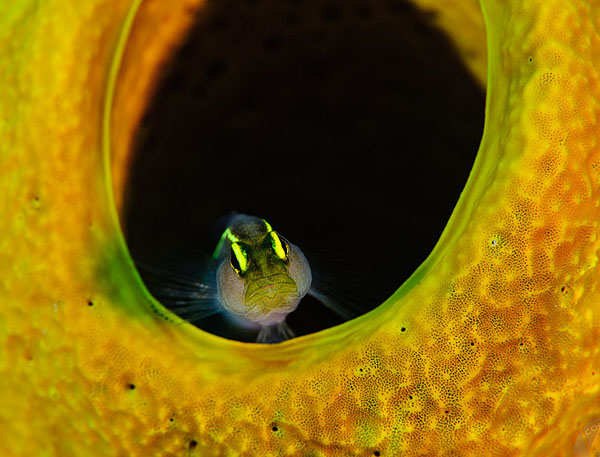
\includegraphics[width=4cm]{img/goby_sponge.jpg}
\end{multicols}
%EndMC


%BeginMC
\question
The ``role'' or ``job'' of a species in a community, represented by all of the resources needed by the species, is called 

\begin{choices}
\correctchoice the niche.%EndChoice
\choice the resource.%EndChoice
\choice a predator.%EndChoice
\choice a predator or prey.%EndChoice
\choice a producer or consumer.%EndChoice
\end{choices}
%EndMC

%BeginMC
\question
A barnacle grows on a whale, doing it no harm. This is an example of

\begin{choices}
\choice predation.%EndChoice
\choice mutualism.%EndChoice
\choice parasitism.%EndChoice
\correctchoice commensalism.%EndChoice
\choice resource partitioning.%EndChoice
\end{choices}
%EndMC

%BeginMC
\question
Based on this food web, which letter represents an organism that could be primary producer? The arrows point \emph{to} the higher trophic levels.

\begin{multicols}{2} 
\begin{choices}
\choice A%EndChoice
\correctchoice B%EndChoice
\choice C%EndChoice
\choice D%EndChoice
\choice E%EndChoice
\end{choices}
\columnbreak
	\hfill 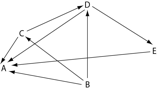
\includegraphics{img/foodweb.png}
\end{multicols}
%EndMC
 
%BeginMC
\question
Which of the following statements about symbiotic relationships is true?

\begin{choices}
\correctchoice A relationship that appears to be commensalism may in fact be mutualistism or parasitism.%EndChoice
\choice Both organisms are harmed in a parasitic relationship.%EndChoice
\choice Both symbiotic organisms usually benefit from the relationship.%EndChoice
\choice The most efficient type of parasite is one that kills its host.%EndChoice
\choice Neither organism benefits in a symbiotic relationship.%EndChoice
\end{choices}
%EndMC

%BeginMC
\question
Malaria is a human disease that occurs when \textit{Plasmodium}, a single-celled organism, invades human blood cells.  The reproduction of \textit{Plasmodium} causes the red blood cells to burst, which decreases the ability of humans to carry oxygen. This is an example of 

\begin{choices}
\choice commensalism.%EndChoice
\choice mutualism.%EndChoice
\correctchoice parasitism.%EndChoice
\choice predation.%EndChoice
\choice symbiosis.%EndChoice
\end{choices}
%EndMC


%BeginMC
\question
According to the figure below, which is most correct about the offspring produced by oysters?

\begin{multicols}{2}
\begin{choices}
\correctchoice Most offspring will die at a very young age.%EndChoice
\choice Most offspring will live most of their natural lifespan.%EndChoice
\choice About the same number of offspring will die every year.%EndChoice
\choice Most offspring will die late in life.%EndChoice
\choice Most offspring will die about half way through their natural life.%EndChoice
\end{choices}
\columnbreak
	\hfill 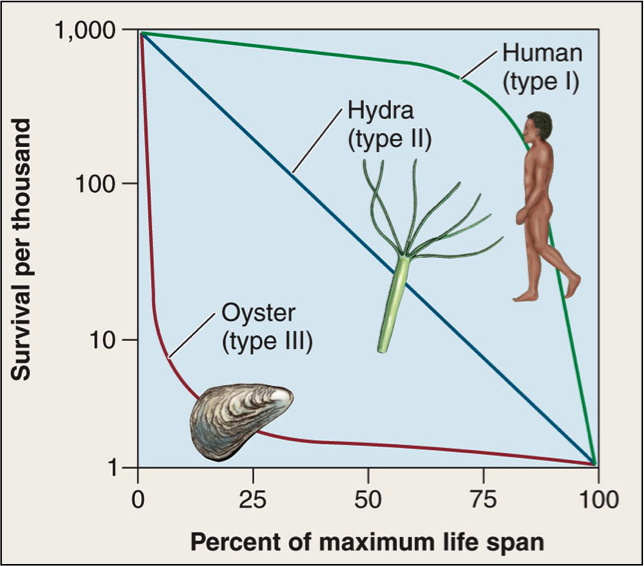
\includegraphics[width=6cm]{img/survivorship.png}
\end{multicols}
%EndMC

%BeginMC
\question
According to the figure below, which is most correct about the offspring produced by hydra?

\begin{multicols}{2}
\begin{choices}
\choice Most offspring will die at a very young age.%EndChoice
\choice Most offspring will live most of their natural lifespan.%EndChoice
\correctchoice About the same number of offspring will die every year.%EndChoice
\choice Most offspring will die late in life.%EndChoice
\choice Most offspring will die about half way through their natural life.%EndChoice
\end{choices}
\columnbreak
	\hfill 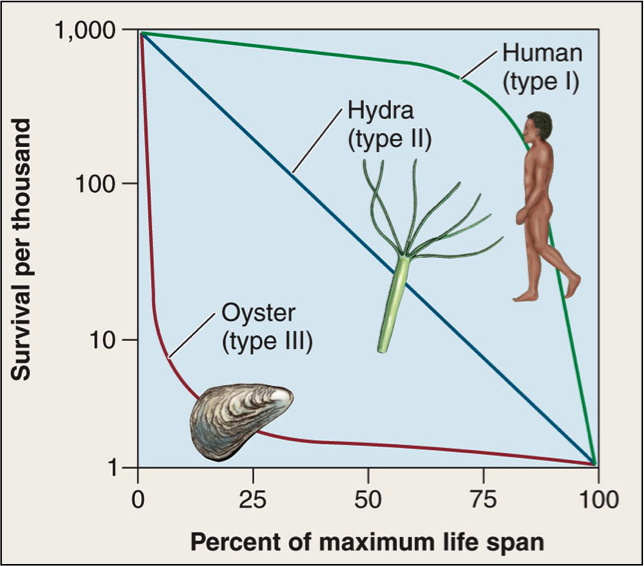
\includegraphics[width=6cm]{img/survivorship.png}
\end{multicols}
%EndMC

%BeginMC
\question
According to the figure below, which is most correct about the offspring produced by Type I organisms?

\begin{multicols}{2}
\begin{choices}
\choice Most offspring will die at a very young age.%EndChoice
\correctchoice Most offspring will live most of their natural lifespan.%EndChoice
\choice About the same number of offspring will die every year.%EndChoice
\choice About 50\% of the individuals will die every year.%EndChoice
\choice Most offspring will die about half way through their natural life.%EndChoice
\end{choices}
\columnbreak
	\hfill 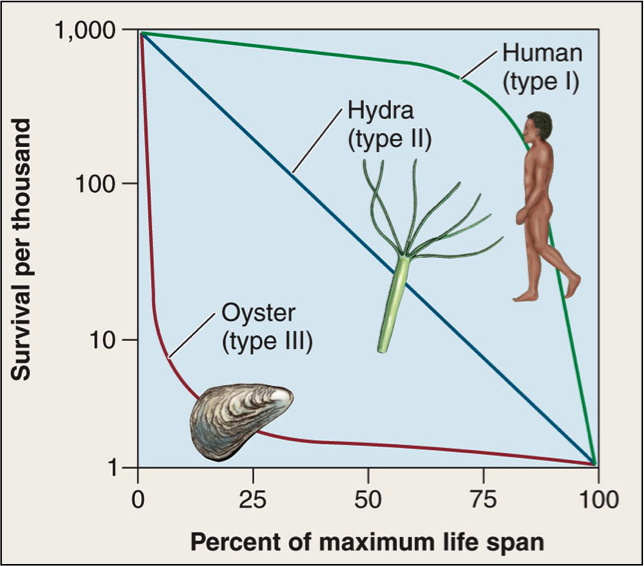
\includegraphics[width=6cm]{img/survivorship.png}
\end{multicols}
%EndMC


%%% --- Community END
%%%%%%%%%%%%%%%%%%%%%%%%%%%%%%%%%%%%%%%%%%%%%%%%%%%%%%%%%%%%%%%%%%%%%%%%%%%%%%
%%%%%%%%%%%%%%%%%%%%%%%%%%%%%%%%%%%%%%%%%%%%%%%%%%%%%%%%%%%%%%%%%%%%%%%%%%%%%%
%%% --- Ecosystems


%% MAKE A QUESTION ABOUT TROPHIC CASCADE

%BeginMC
\question
The land on the south side of the Himalayan mountain range (below) receives relatively high levels of rainfall and has fertile farmlands.  The land north of the mountain range is hot and dry and can't be farmed.  Which of the following is true.

\begin{multicols}{2}
\begin{choices}
\choice The south side of the Himalayan mountain range is in a rain shadow.%EndChoice
\choice The desert in southern China warms the north side of the mountain range, causing it to dry out.%EndChoice
\choice The cool, moist Indian Ocean air heats up as it rises, releasing its precipitation as it passes the tops of the mountains, and this warm, now dry air cools as it descends on the leeward side of the range.%EndChoice
\correctchoice Warm, moist air from the Indian Ocean blows north, rises and cools, releasing precipitation as it moves up the south side of the range, and this cool, now dry air mass heats up as it descends on the north side of the range.%EndChoice
\choice The warm, moist air is too dense to rise over the height of Mount Everest and the other mountains in this range so the moisture remains on the south side of the range.%EndChoice
\end{choices}
\columnbreak
	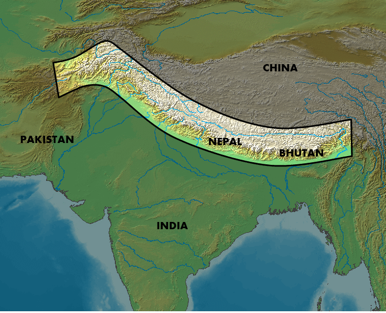
\includegraphics[width=8cm]{img/himalayas.png}
\end{multicols}
%EndMC


%BeginMC
\question
Higher elevations on a mountain experience less precipitation and cooler temperatures than low elevations.  As you descended from the top of the mountain, you would notice a change in the types of plants and animals present in the community.  This is analogous to the changes in the ecosystems if you walked 

\begin{choices}
\correctchoice from the north pole to the equator.%EndChoice
\choice east to west over different altitudes.%EndChoice
\choice west to east at one latitude.%EndChoice
\choice from the equator to the south pole.%EndChoice
\choice from the north pole to the south pole.%EndChoice
\end{choices}
%EndMC


%BeginMC
\question
In 2011, the Mississippi River experienced a record flood event.  Which of the following statements is the best prediction of how this record flood event will affected the Gulf of Mexico dead zone that summer?

\begin{choices}
\correctchoice The dead zone will be larger because the volume of water will carry even more nutrients into the Gulf of Mexico.%EndChoice
\choice The dead zone will be smaller because the volume of water will bring more oxygen to the Gulf of Mexico, which will offset the hypoxia.%EndChoice
\choice The dead zone will be smaller because the volume of water will dilute the nutrients, reducing eutrophication.%EndChoice
\choice The dead zone will be similar to previous years because most of the flood water will soak into the ground and not enter the Gulf of Mexico.%EndChoice
\choice The dead zone will be larger because the volume of water will cause more fishes to avoid the freshwater input.%EndChoice
\end{choices}
%EndMC


%BeginMC
\question
The southeastern region of Missouri lies within the temperate broadleaf forest ecosystem. According to the climograph below, the temperate broadleaf forest

\begin{multicols}{2} 
\begin{choices}
\choice never has more than about 220 cm (87 inches) of rainfall per year.%EndChoice
\correctchoice has an average of 60--220 cm of precipitation per year.%EndChoice
\choice has more rain and similar temperatures to the northern coniferous forest.%EndChoice
\choice always has more precipitation than the temperate grassland.%EndChoice
\choice is never warmer than the temperate grassland.%EndChoice
\end{choices}
\columnbreak
	\hfill 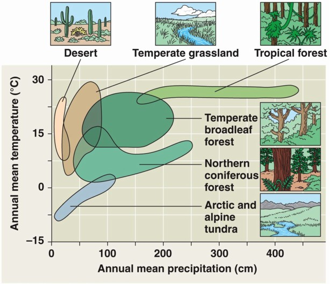
\includegraphics[width=6cm]{img/climograph.png}
\end{multicols}
%EndMC



%BeginMC
\question
In ecosystems, why is ``cycling'' used to describe the transfer of chemical elements and nutrients, but the ``flow'' is used for the transfer of energy?

\begin{choices}
\correctchoice Chemical elements are recycled within ecosystems, but energy flows through and out of ecosystems.%EndChoice
\choice Both chemical elements and energy are recycled but can flow to other ecosystems.%EndChoice
\choice Chemical elements are cycled into ecosystems from other ecosystems, but energy constantly flows within the ecosystem.%EndChoice
\choice Both chemical elements and energy flow within an ecosystem but can cycle to other ecosystems.%EndChoice
\choice Energy flows from one ecosystem to other ecosystems, but chemical elements constantly cycle within an ecosystem.%EndChoice
\end{choices}
%EndMC


%BeginMC
\question
Ecologists say that energy ``flows'' through an ecosystem because

\begin{choices}
\choice energy, like air, can be thought of as a fluid that moves through the ecosystem.%EndChoice
\correctchoice the heat energy that is created by metabolism can never again enter the ecosystem.%EndChoice
\choice energy flows from high trophic levels, such as top predators, to low trophic levels, such as prey.%EndChoice
\choice energy cycles from one trophic level to the next.%EndChoice
\choice all energy that enters an ecosystem flows there from the sun.%EndChoice
\end{choices}
%EndMC

%BeginMC
\question
In the Gulf of Mexico, eutrophication causes

\begin{choices}
\choice the size of the Dead Zone to increase because of the loss of nutrients.%EndChoice
\correctchoice the community of marine algae to increase due to added nutrients.%EndChoice
\choice the community of marine algae to die due to the loss of nutrients.%EndChoice
\choice the number of shrimp to decrease due to the loss of nutrients.%EndChoice
\choice the number of shrimp to increase due to added nutrients.%EndChoice
\end{choices}
%EndMC

%BeginMC
\question
The dead zone in the Gulf of Mexico and other oceans around the globe occurs when

\begin{choices}
\choice an excess of nutrients causes an algal bloom. The algae consume all of the oyxgen in the water for photosynthesis, so other organisms can no longer live there.%EndChoice
\choice eutrophication causes an absence of nutrients in the zone.%EndChoice
\choice commercial fishers overharvest shrimp, crab, fishes and other sea animals.%EndChoice
\correctchoice an excess of nutrients causes an algal bloom, followed by death of the algae. Decomposition of the algae uses up the oxygen in the water, so other organisms can no longer live there.%EndChoice
\choice global climate change causes the water to become too warm to sustain life.%EndChoice
\end{choices}
%EndMC


%BeginMC
\question
The number of herbivores found in an ecological pyramid is limited by the

\begin{choices}
\choice number of producers below the herbivores.%EndChoice
\choice number of predators that eat the herbivores.%EndChoice
\correctchoice amount of energy transferred from producers to the next trophic level.%EndChoice
\choice amount of energy in the entire pyramid.%EndChoice
\choice number of trophic levels (e.g., 3 or 4 levels) above the herbivores.%EndChoice
\end{choices}
%EndMC

%BeginMC
\question
The major abiotic (non-living) components of ecosystems include

\begin{choices}
\correctchoice temperature, moisture, sunlight, and nutrients.%EndChoice
\choice plants, animals, climate, and microorganisms.%EndChoice
\choice producers, herbivores, carnivores, and plants.%EndChoice
\choice consumers, detritus feeders, decomposers, and parasites.%EndChoice
\choice producers, consumers, decomposers, and detritus feeders.%EndChoice
\end{choices}
%EndMC

%BeginMC
\question
In general, more herbivores will be found in an ecosystem than carnivores. Why?

\begin{choices}
\correctchoice There is more total energy at the primary consumer trophic level to support more biomass.%EndChoice
\choice There is more total energy at the secondary consumer trophic level to support larger but fewer carnivores.%EndChoice
\choice More energy is transferred from primary producers to primary consumers than from primary consumers to secondary consumers.%EndChoice
\choice Herbivores are usually faster than carnivores so they survive longer and reproduce more often.%EndChoice
\choice More energy is transferred from plants to herbivores than from herbivores to carnivores.%EndChoice
\end{choices}
%EndMC

%BeginMC
\question
Lower elevations on a very high mountain near the equator experience more precipitation and warmer temperatures than high elevations. If you climbed from the base of the mountain to the top, you would notice a change in the types of ecosystems present on the mountain side. This would be similar to the changes (Note: The equator is 0$^\circ$, the poles are at 90$^\circ$). 

\begin{choices}
\choice traveling across South American from 55$^\circ$ south latitude to 5$^\circ$ south latitude.%EndChoice
\correctchoice traveling across North America from 15$^\circ$ north latitude to 55$^\circ$ north latitude.%EndChoice
\choice traveling across South America and North American from 55$^\circ$ south latitude to 55$^\circ$ north latitude.%EndChoice
\choice across Europe and Asia from 15$^\circ$ east longitude to 15$^\circ$ west longitude.%EndChoice
\choice across Europe and Asia from 15$^\circ$ west longitude to 15ï$^\circ$ east longitude.%EndChoice
\end{choices}
%EndMC


%BeginMC
\question
Which of the following is an example of an ecosystem?

\begin{choices}
\choice All of the brook trout in a 500 hectare2 river drainage system.%EndChoice
\correctchoice The plants, animals and decomposers, plus the nutrients and rainfall in a tropical rain forest.%EndChoice
\choice The plants, animals, and decomposers that inhabit an alpine meadow.%EndChoice
\choice A pond and all of the plant and animal species that live in it.%EndChoice
\choice The intricate interactions of the various plant and animal species on a savanna during a drought.%EndChoice
\end{choices}
%EndMC

%BeginMC
\question
Probably the most important factor(s) affecting the distribution of ecosystems is (are)

\begin{choices}
\correctchoice climate.%EndChoice
\choice wind and ocean water current patterns.%EndChoice
\choice wind direction and rain shadows.%EndChoice
\choice longitude and latitude.%EndChoice
\choice day length and rainfall.%EndChoice
\end{choices}
%EndMC

%BeginMC
\question
In summer 2012, the Midwest experienced one of the worst droughts in recorded history. Which of the following statements is the best explanation of how this drought affected the Gulf of Mexico dead zone during summer 2012?

\begin{choices}
\correctchoice The dead zone will be smaller because the Mississippi River will carry less water so fewer nutrients will be carried to the Gulf of Mexico.%EndChoice
\choice The dead zone will be smaller because farmers, anticipating the drought, would not have added fertilizer to the crop fields the spring before the drought.%EndChoice
\choice The dead zone will be similar to previous years because the drought is not likely to affect the amount of water that flows out through the Mississippi River.%EndChoice
\choice The dead zone will be larger because the reduced volume of water will concentrate the nutrients that enter the Gulf of Mexico.%EndChoice
\choice The dead zone will be smaller because less freshwater will enter the Gulf of Mexico, allowing more saltwater fishes to live around the mouth of the river.%EndChoice
\end{choices}
%EndMC

%BeginMC
\question
On average, the amount of primary consumer biomass is about \underline{\hspace{2cm}} less than the amount of primary producer biomass.

\begin{choices}
\choice 10\%%EndChoice
\choice 20\%%EndChoice
\choice 50\%%EndChoice
\choice 80\%%EndChoice
\correctchoice 90\%%EndChoice
\end{choices}
%EndMC


%BeginMC
\question
On average, the amount of secondary consumer biomass is about \underline{\hspace{2cm}} less than the amount of primary producer biomass. 
\begin{choices}
\choice 10$\times$%EndChoice
\choice 20$\times$%EndChoice
\choice 50$\times$%EndChoice
\choice 80$\times$%EndChoice
\correctchoice 100$\times$%EndChoice
\end{choices}
%EndMC

%BeginMC
\question
On average, the amount of secondary consumer biomass is about \underline{\hspace{2cm}} less than the amount of primary producer biomass. 
\begin{choices}
\choice 10\times%EndChoice
\choice 20\times%EndChoice
\choice 50\times%EndChoice
\choice 80\times%EndChoice
\correctchoice 100\times%EndChoice
\end{choices}
%EndMC



%BeginMC
\question
The microscopic algae community in the Gulf of Mexico is limited by which of the following nutrients?

\begin{choices}
\choice carbon%EndChoice
\choice \ce{CO2}%EndChoice
\choice hydrogen%EndChoice
\choice oxygen%EndChoice
\correctchoice nitrogen%EndChoice
\end{choices}
%EndMC

%BeginMC
\question
A transient killer whale eats seals. The seals ate fish. The fish ate part of a dead killer whale laying on the sea floor, but also ate smaller live squid. You do not know what the squid might have eaten. The fish in this example is acting as \underline{\hspace{2cm}}. (Choose the best answer)

\begin{choices}
\correctchoice a consumer and a decomposer.%EndChoice
\choice a secondary consumer and a primary consumer.%EndChoice
\choice a secondary consumer and a decomposer.%EndChoice
\choice a secondary consumer, a decomposer, and a consumer one trophic level higher than the killer whale.%EndChoice
\choice a consumer and a producer.%EndChoice
\end{choices}
%EndMC

%BeginMC
\question
The downwind side of large mountain ranges is often drier than the upwind side. This phenomenon occurs because

\begin{choices}
\choice mountains are always near oceans.%EndChoice
\choice because the rainforest on the west side of the mountain absorbs all of the rain out of the air before it crosses the mountain.%EndChoice
\choice when the desert on the east side of the mountains sucks the moisture out of the air.%EndChoice
\correctchoice the mountain range deflects the moisture-laden air from the ocean up into the atmosphere. The air cools and drops its moisture as rain. The now-dry air flows across downwind side of the mountains.%EndChoice
\choice the wind blows the moisture out of the air before it can cross the mountains.%EndChoice
\end{choices}
%EndMC

%BeginMC
\question
Energy from the sun is converted into chemical energy for organisms by

\begin{choices}
\correctchoice producers.%EndChoice
\choice carnivores.%EndChoice
\choice decomposers.%EndChoice
\choice detritivores.%EndChoice
\choice herbivores.%EndChoice
\end{choices}
%EndMC

%BeginMC
\question
Plants produce water vapor during photosynthesis, which goes from the plant to the atmosphere. The water vapor in the atmosphere eventually falls back to the earth as rain. This process would be part of

\begin{choices}
\correctchoice the water cycle.%EndChoice
\choice energy flow.%EndChoice
\choice plant metabolism.%EndChoice
\choice the entire ecosystem.%EndChoice
\choice the energy cycle.%EndChoice
\end{choices}
%EndMC

%BeginMC
\question
The energy that is \textit{not} transferred to other trophic levels, detritivores or decomposers is lost

\begin{choices}
\correctchoice as metabolic heat.%EndChoice
\choice in fecal matter.%EndChoice
\choice to consumers at any trophic level.%EndChoice
\choice to primary consumers.%EndChoice
\choice to secondary consumers.%EndChoice
\end{choices}
%EndMC


%BeginMC
\question
The Mediterranean coast and coastal California have similar types of ecosystems. This is because

\begin{choices}
\correctchoice they have similar climates.%EndChoice
\choice they have similar types of organisms.%EndChoice
\choice they are both wine-growing regions.%EndChoice
\choice they have similar types of communities.%EndChoice
\choice they are at similar latitudes.%EndChoice
\end{choices}
%EndMC



%%% --- Ecosystems END
%%%%%%%%%%%%%%%%%%%%%%%%%%%%%%%%%%%%%%%%%%%%%%%%%%%%%%%%%%%%%%%%%%%%%%%%%%%%%%
